\documentclass[final, letterpaper, 12pt]{article}

\usepackage{booktabs}
\usepackage{enumerate}
\usepackage{enumitem}
\usepackage[hypcap]{caption}
\usepackage[spanish,es-tabla]{babel}
\usepackage[utf8]{inputenc}
\usepackage{graphicx}
\usepackage{amsthm}
\usepackage{eufrak}
\usepackage{amsmath}
\usepackage[justification=centering]{caption}
\usepackage{multirow}
\usepackage{mathrsfs} % para formato de letra
\usepackage{amssymb, amsmath, amsbsy} % simbolitos
\usepackage{listings}
\usepackage[compatibility=false]{caption}
\usepackage{color}
%\usepackage{xcolor}
%\usepackage{inconsolata}
\usepackage[T1]{fontenc}
\usepackage{longtable}
\usepackage{fancyhdr}
\usepackage{lmodern}
\usepackage{import}
\usepackage{float}
\usepackage[margin=1.1in, foot=30pt, head = 30pt, bottom = 1.3in]{geometry}
\usepackage{hyphenat}
\usepackage[document]{ragged2e}
\usepackage{array}
\usepackage{epstopdf}
\usepackage{imakeidx}
\usepackage[bookmarks=true, hidelinks]{hyperref}
\usepackage{bookmark}
\usepackage{titlesec}
\usepackage{siunitx}
\usepackage{subcaption}
\usepackage{gensymb}
\usepackage{setspace}



\titleclass{\subsubsubsection}{straight}[\subsection]

\newcounter{subsubsubsection}[subsubsection]
\renewcommand\thesubsubsubsection{\thesubsubsection.\arabic{subsubsubsection}}
\renewcommand\theparagraph{\thesubsubsubsection.\arabic{paragraph}} % optional; useful if paragraphs are to be numbered
\newtheorem{defi}{{\it Definición}}[subsection]
\newtheorem{ejemplo}{{\it Ejemplo}}[subsection]
\newtheorem{teo}{{\it Teorema}}[subsection]
\newtheorem{prop}{{\it Proposición}}[subsection]
\newtheorem{coro}{{\it Corolario}}[subsection]
\newtheorem{lema}{{\it Lema}}[subsection]
\newtheorem{lema}{{\it Lema}}

\titleformat{\subsubsubsection}
  {\normalfont\normalsize\bfseries}{\thesubsubsubsection}{1em}{}
\titlespacing*{\subsubsubsection}
{0pt}{3.25ex plus 1ex minus .2ex}{1.5ex plus .2ex}

\makeatletter
\renewcommand\paragraph{\@startsection{paragraph}{5}{\z@}%
  {3.25ex \@plus1ex \@minus.2ex}%
  {-1em}%
  {\normalfont\normalsize\bfseries}}
\renewcommand\subparagraph{\@startsection{subparagraph}{6}{\parindent}%
  {3.25ex \@plus1ex \@minus .2ex}%
  {-1em}%
  {\normalfont\normalsize\bfseries}}
\def\toclevel@subsubsubsection{4}
\def\toclevel@paragraph{5}
\def\toclevel@paragraph{6}
\def\l@subsubsubsection{\@dottedtocline{4}{7em}{4em}}
\def\l@paragraph{\@dottedtocline{5}{10em}{5em}}
\def\l@subparagraph{\@dottedtocline{6}{14em}{6em}}
\makeatother

\setcounter{secnumdepth}{4}
\setcounter{tocdepth}{4}

\graphicspath{{./img/}}

\newcolumntype{P}[1]{>{\centering\arraybackslash}p{#1}}

\definecolor{darkblue}{rgb}{0,0,0.6}
\definecolor{darkgray}{rgb}{0.3,0.3,0.3}
\definecolor{lightgray}{rgb}{0.98,0.98,0.98}

\lstset{literate=
  {á}{{\'a}}1 {é}{{\'e}}1 {í}{{\'i}}1 {ó}{{\'o}}1 {ú}{{\'u}}1
  {Á}{{\'A}}1 {É}{{\'E}}1 {Í}{{\'I}}1 {Ó}{{\'O}}1 {Ú}{{\'U}}1
  {à}{{\`a}}1 {è}{{\`e}}1 {ì}{{\`i}}1 {ò}{{\`o}}1 {ù}{{\`u}}1
  {À}{{\`A}}1 {È}{{\'E}}1 {Ì}{{\`I}}1 {Ò}{{\`O}}1 {Ù}{{\`U}}1
  {ä}{{\"a}}1 {ë}{{\"e}}1 {ï}{{\"i}}1 {ö}{{\"o}}1 {ü}{{\"u}}1
  {Ä}{{\"A}}1 {Ë}{{\"E}}1 {Ï}{{\"I}}1 {Ö}{{\"O}}1 {Ü}{{\"U}}1
  {â}{{\^a}}1 {ê}{{\^e}}1 {î}{{\^i}}1 {ô}{{\^o}}1 {û}{{\^u}}1
  {Â}{{\^A}}1 {Ê}{{\^E}}1 {Î}{{\^I}}1 {Ô}{{\^O}}1 {Û}{{\^U}}1
  {œ}{{\oe}}1 {Œ}{{\OE}}1 {æ}{{\ae}}1 {Æ}{{\AE}}1 {ß}{{\ss}}1
  {ű}{{\H{u}}}1 {Ű}{{\H{U}}}1 {ő}{{\H{o}}}1 {Ő}{{\H{O}}}1 {ñ}{{\~n}}1
  {ç}{{\c c}}1 {Ç}{{\c C}}1 {ø}{{\o}}1 {å}{{\r a}}1 {Å}{{\r A}}1
  {€}{{\EUR}}1 {£}{{\pounds}}1
}

\lstset{
    language=Matlab, % choose the language of the code
    basicstyle=\fontfamily{pcr}\selectfont\footnotesize\color{black},
    keywordstyle=\color{darkblue}\bfseries, % style for keywords
    numbers=none, % where to put the line-numbers
    numberstyle=\tiny, % the size of the fonts that are used for the line-numbers     
    backgroundcolor=\color{lightgray},
    showstringspaces=false, % underline spaces within strings
    showtabs=false, % show tabs within strings adding particular underscores
    frame=single, % adds a frame around the code
    tabsize=2, % sets default tabsize to 2 spaces
    rulesepcolor=\color{gray},
    rulecolor=\color{black},
    captionpos=b, % sets the caption-position to bottom
    breaklines=true, % sets automatic line breaking
    breakatwhitespace=false,
    inputencoding=utf8,
    extendedchars=true,
    commentstyle= \color{gray}\itshape,
    inputpath=code,
}

\DeclareCaptionFont{white}{ \color{white} }
\DeclareCaptionFormat{listing}{
  \colorbox[cmyk]{0.43, 0.35, 0.35,0.01 }{
    \parbox{\textwidth}{\hspace{15pt}#1#2#3}
  }
}
\captionsetup[lstlisting]{ format=listing, labelfont=white, textfont=white, singlelinecheck=false, margin=0pt, font={bf,footnotesize} }



% Turn on the style
\pagestyle{fancy}
% Clear the header and footer
\fancyhead{}
\fancyfoot{}
\fancyhead{}
% Set the right side of the footer to be the page number
\fancyfoot[R]{\thepage}

\begin{document}


%%%%%%%%%%%%%%%%%%%%%%%%% Portada %%%%%%%%%%%%%%%%%%%%%%%%%%%%%
\justifying
\begin{titlepage}

\begin{figure}[t]

\includegraphics[width=0.33\linewidth]{Imagenes/1MAIN/logo-usm-g.jpg} \hspace{4.8cm}

\includegraphics[width=0.33\linewidth]{Imagenes/1MAIN/logo_mat.png}\\[3.2cm]
\end{figure}

\begin{center}
\Huge{ \bfseries{Trabajo de Investigación\\[1.1cm]
Extensiones de cuerpos. Monomorfismos de cuerpos. La norma y la traza. Discriminante\\[1.8cm]}}
\end{center}

\begin{table}[h]
\centering
\begin{tabular}{ll}
\textbf{Fecha}       & 28/6/2019                          \\
\textbf{Integrantes} & Roberto Gonzalez          \\
                     & Matias Alvarez             \\
                     & Francisco Nilsson              \\
\multicolumn{2}{l}{}                                       \\
\textbf{Asignatura}  & Algebra Lineal \\
\textbf{Profesores}  & Gonzalo Riquelme  \\                   
\end{tabular}
\end{table}

\vspace{1.5cm}
\begin{center}
\end{center}
\end{titlepage}

%%%%%%%%%%%%%%%%%%%%%%%%%%%%%%%%%%%%%%%%%%%%%%%%%%%%%%%%%%
\newpage
%%%%%%%%%%%%%%%%%%%%%%%% Índice %%%%%%%%%%%%%%%%%%%%%%%%%%

%\pdfbookmark{\contentsname}{Contents}
\tableofcontents

%\cleardoublepage
\newpage

\addcontentsline{toc}{section}{Índice de figuras} % para que aparezca en el indice de contenidos
\listoffigures % indice de figuras

%\cleardoublepage
\addcontentsline{toc}{section}{Índice de tablas} % para que aparezca en el indice de contenidos
\listoftables % indice de tablas
%%%%%%%%%%%%%%%%%%%%%%%%%%%%%%%%%%%%%%%%%%%%%%%%%%%%%%%%%%


\newpage

%%%%%%%%%%%%%%%%%%%%%%%% Estructura %%%%%%%%%%%%%%%%%%%%%%%%%%
\mainmatter
\pagenumbering{arabic}
%--------------------------------
% SIN TERMINAR
%--------------------------------

\section{Introducción}
\vspace{2mm}

\subsection{Propósito}

\begin{itemize}
\item 
\item 
\item 
\end{itemize}

\subsection{Referencias}
\begin{itemize}
    \item Labra, A., & Suazo, A. (2011). Elementos de la teoría de cuerpos. Santiago, Chile: J.C. Sáez Editor.
    \item Pantoja, J. Teoría de Galois. Apuntes. 
    \item Lang, S. (2012). Linear Algebra (3ª ed.). Nueva York, Estados Unidos: Springer New York.
\end{itemize}
 
\newpage

\section{Anillos y cuerpos}
\subsection{Definiciones y resultados básicos}
\begin{defi}
Sea R un conjunto no vació, en el que están definidas dos operaciones: suma y multiplicación ($+ \land \times$). Diremos que $(R,+,\times)$ es un anillo si y sólo si:
\begin{enumerate}
    \item $(R,+)$ es un grupo abeliano. Además, para todo $a,b,c \in R$:
    \item $a\times b\in R$,
    \item $(a\times b)\times c = a\times (b\times c),$,
    \item $a\times (b\times c) = a\times b + a\times c$ y $(b+c)\times a = b\times a + c\times a$.
\end{enumerate}
\end{defi}
\begin{ejemplo}
El conjunto de los números enteros $Z$ tiene la estructura algebraica de un anillo. Además, es un anillo conmutativo y con elemento unidad, que es precisamente el 1.
\end{ejemplo}
Se dice que un anillo es conmutativo, si $a\times b = b\times a$ para todo $a,b\in R$. Si existe un elemento denotado por 1 en $R$ tal que $1\times a = a\times 1 = a$ para todo $a\in R$, se dice que es un anillo con elemento unidad.
\begin{defi}
Si $R$ es un anillo conmutativo con elemento unidad $1\neq 0$ tal que todos los elementos no nulos de $R$ admiten inversos multiplicativos en $R$, entonces diremos que $R$ es un cuerpo.
\end{defi}
Sea $F$ un cuerpo. Notemos que el inverso multiplicativo del 0 no existe, por lo tanto, para $(F,\times)$ esta definida para todo elemento en $F-\lbrace 0\rbrace$.
\begin{defi}
Si $S$ es un subconjunto de un anillo $R$ y $S$ es un anillo con las mismas operaciones sumas y multiplicación de $R$, entonces se dice que $S$ es un subanillo de $R$.
\end{defi}
Para demostrar que un subconjunto de un anillo $R$ es un anillo, se puede utilizar el siguiente lema, que es bastante análogo a la hora de demostrar si un subconjunto es un subespecie vectorial.
\begin{lema}
Un subconjunto $S$ de un anillo $R$ es un subanillo de $R$, si y sólo si,
\begin{enumerate}
    \item $0\in S$,
    \item para todo $a,b\in S:a-b\in S$,
    \item para todo $a,b\in S:ab\in S$,
\end{enumerate}
\end{lema}
\begin{ejemplo}
El conjunto de los números enteros $Z$ tiene la estructura algebraica de un anillo. Además, es un anillo conmutativo y con elemento unidad, que es precisamente el 1.
\end{ejemplo}
Un anillo $R$ es conmutativo, si $a\times b = b\times a$ para todo $a,b\in R$. Si existe un elemento denotado como 1 en R tal que $1\times a=a\times 1 = a$ para todo $a\in R$, entonces el anillo $R$ es unitario o con elemento unidad.
\begin{defi}
Si $R$ es un anillo conmutativo con elemento unidad $1\neq 0$ tal que todos los elementos no nulos de $R$ admiten inversos multiplicativos en $R$, entonces diremos que $R$ es un cuerpo.
\end{defi}
Notemos que $(R,\times)=(R,+)-\lbrace 0 \rbrace$, pues el elemento 0 es el único elemento que no posee un inverso multiplicativo.
\begin{ejemplo}
El conjunto de los números enteros $Z$ no es un cuerpo, pues no posee inversos multiplicativos para todo elemento no nulo en $Z$, pero los números racionales $Q$ si son un cuerpo, pues todo elemento en $Q$ posee un inverso multiplicativo.
\end{ejemplo}
\begin{defi}
Si $S$ es un subconjunto de un anillo $R$ y $S$ es un anillo con las mismas operaciones suma y multiplicación de $R$, entonces se dice que $S$ es un subanillo de R.
\end{defi}
La definición anterior es bastante análoga a la definición de un subespacio vectorial, tal como se ha visto en clases. También se puede definir de otra manera, con el lema posterior.
\begin{defi}
Un subconjunto $S$ de un anillo $R$ es un subanillo de $R$, si y sólo si,
\begin{enumerate}
    \item $0\in S$,
    \item para todo $a,b\in S: a-b\in S$,
    \item para todo $a,b\in S: ab\in S$.
\end{enumerate}
\end{defi}
Los siguientes ejemplos de anillos serán los mas utilizados en este trabajo de investigación, los cuales son:
\begin{enumerate}
    \item El conjunto $Z[x]$ de todos los polinomios con coeficientes en $Z$, con las operaciones usuales de suma y multiplicación de polinomios, es un dominio de integridad.
    \item El conjunto $Z[i]=\lbrace a+bi/a,b\in Z \rbrace$, donde $i$ es el numero complejo, con las operaciones usuales de suma y multiplicación de números complejos, es un dominio de integridad.
\end{enumerate}
Un anillo $R$ es un dominio de integridad, si es un anillo conmutativo y con elemento unidad $(1\neq 0)$ y sin divisores del cero. Un elemento es un divisor de cero, si existe un elemento no nulo $b\in R$ tal que $a\times b = 0$.
\begin{defi}
Un subconjunto $U$ de un anillo $R$, se dice que es un ideal de $R$, si:
\begin{enumerate}
    \item $0\in U$,
    \item para todo $a,b\in U:a-b\in U$,
    \item para todo $u\in U$ y $r\in R : ur\in U$ y $ru\in R$.
\end{enumerate}
\end{defi}
\begin{ejemplo}
El conjunto $Z[i]$, con las operaciones usuales de suma y multiplicación de números complejos, es un subanillo de $C$, pero $Z[i]$ no es ideal de $C$.
\end{ejemplo}
\begin{teo}
Sea $R$ un anillo conmutativo con elemento unidad y $a_{1},...,a_{k}$ elementos en $R$. Entonces el conjunto $U=\lbrace a_{1}x_{1}+...+a_{k}x_{k}/x_{1},...,x_{k}\in R \rbrace$ es un ideal de $R$. Se dice que $U$ es el ideal de $R$ generado por los elementos $a_{1},...,a_{k}$ y se denota $U=\langle a_{1},...,a_{k} \rangle$.
\end{teo}
\begin{defi}
Sea $R$ un anillo conmutativo con elemento unidad. Diremos que $R$ es un anillo de ideales principales, si para cada ideal $U$ de $R$ existe un elemento $a\in R$ tal que $U = \langle a \rangle = \lbrace ax / x\in R \rbrace$.
\end{defi}
\begin{lema}
Si $U, V$ son ideales de un anillo $R$, entonces $U+V=\lbrace u+v/u\in U,v\in V\rbrace$ es un ideal de $R$.
\end{lema}
\begin{ejemplo}
En $Z$, $\langle 2,5 \rangle = \langle 1 \rangle = Z$, ya que, $3\times 2 + (-1)\times 5 = 1$, por lo tanto, es un ideal principal.
\end{ejemplo}
\begin{defi}
Si un subconjunto $F$ de un cuerpo $K$, con las mismas operaciones de suma y producto de $K$, es un cuerpo, entonces diremos que $F$ es un subcuerpo de $K$ (denotado por $F\leq Q$).
\end{defi}
Nuevamente, tal como sucede en álgebra lineal, existe un lema que permite demostrar lo anterior:
\begin{lema}
Sea $K$ un cuerpo y $F$ un subconjunto de $K$. Entonces $F$ es un subcuerpo de $K$, si y sólo si,
\begin{enumerate}
    \item $0\in F$,
    \item para todo $a,b\in F : a-b\in F$ y $ab\in F$,
    \item $1\in F$ es un elemento en $F$,
    \item para todo elemento no nulo en $F$ el inverso multiplicativo está en $F$.
\end{enumerate}
\end{lema}
\begin{ejemplo}
Se demostrará que $Q(i)=\lbrace a+bi/a,b\in Q \rbrace$ es un subcuerpo de $C$. 
\begin{enumerate}
    \item $0 = 0 + 0i \in Q(i)$.
    \item Sean $a+bi$, $c+di$ con $a,b,c,d\in Q$. Entonces
    \[(a+bi)-(c+di)=(a-c)+(b-d)i\in Q(i)\]
    y
    \[(a+bi)(c+di)=(ac-bd)+(ad+bc)i \in Q(i)\].
    \item $1=1+0i\in Q(i)$.
    \item Sea $a+bi \neq 0$ con $a,b\in Q$. Entonces $a\neq 0$ o $b\neq 0$, de donde $a^{2}+b^{2}>0$. El inverso multiplicativo de $a+bi$ es 
    \[(a+bi)^{-1}=\frac{a}{a^{2}+b^{2}}-\frac{b}{a^{2}+b^{2}}i\in Q(i)\].
\end{enumerate}
\end{ejemplo}
Consideremos a continuación un ideal $U$ de un anillo $R$. Dado que $(U,+)$ es un subgrupo de $(R,+)$, se puede definir el conjunto $R/U=\lbrace a+U/a\in R \rbrace$. De acuerdo a la teoria de grupos, el conjunto $R/U$ es un grupo bajo la adición donde 
\[(a+U)+(b+U)=(a+b)+U\]
para todo $a,b \in R$. Mientras que la multiplicación esta definida como
\[(a+U)(b+U)=ab+U\]
para todo $a,b\in R$. Este anillo es conocido como el anillo cuociente de $R$ por $U$.
\begin{defi}
Sea $R$ una anillo. Un ideal $M$ de $R$ con $M\neq R$ se dice que es un ideal maximal de $R$, si dado un ideal $U$ de $R$ tal que $M\subset U \subset R$, entonces $M=U$ o $U=R$. Es decir, no existe un ideal $U$ de $R$ tal que $M\subsetneq U \neq R$.
\end{defi}
\begin{ejemplo}
Demostraremos que el ideal $<7>=7Z$ de $Z$ es un ideal maximal de Z.
Sea un U ideal de $Z$ tal que $7Z\subset U \subset Z$. Como $Z$ es un anillo de ideales principales y $U\neq \lbrace 0 \rbrace (7\in U)$, entonces existe $n\in Z^{+}$ tal que $U=nZ$. Dado que $7Z\subset  nZ$, entonces existe $n\in Z^{+}$ tal que $7=nq$. Lo anterior implica que $n=7$ o $n=1$. Si $n=7$, entonces $7Z=U$ y si $n=1$, entonces $U=Z$. Por lo tanto, $7Z$ es un ideal maximal de $Z$.
\end{ejemplo}
Del ejemplo anterior, se puede observar que el ideal $pZ$ sera maximal, si y sólo si, p es un numero primo. Esto se puede ver intuitivamente en el ejemplo.\\
El siguiente teorema es fundamental para la teoría de cuerpos, pues permite la construcción de un cuerpo a partir de un anillo conmutativo con elemento unidad y de un ideal maximal de anillos.
\begin{teo}
Sea $R$ un anillo conmutativos son elemento unidad $1\neq 0$ y $M$ un ideal de $R$. Entonces $M$ un ideal maximal de $R$, si y sólo si, $R/M$ es un cuerpo.
\begin{proof}
Supongamos que $M$ es un ideal maximal de $R$. Debemos mostrar que $R/M$ es un anillo conmutativo con elemento unidad tal que todos los elementos no nulos en $R/M$  admiten inversos multiplicativos en $R/M$.\\
Sabemos que $R/M$ es un anillo conmutativo con elemento unidad $1+M\neq 0+M$. Se probará a continuación que, si $a+M\in R/M$ con $a+M\neq 0+M$, o sea $a\notin M$, entonces $a+M$ no tiene inverso multiplicativo en $R/M$. Ahora, $\langle a \rangle$ y $M$ son ideales de $R$ y por el lema 2.1.2, $M+\langle a \rangle$ es un ideal de $R$.
Como $a\notin M$ y $a=0+a\in M+\langle a \rangle$, entonces $M\subsetneq M+\langle a \rangle$. Por hipótesis, $M$ es un ideal maximal de R, por lo tanto, se debe tener que $M+\langle a \rangle = R$. Dado que $1\in R$, entonces existen $m\in M$ y $b\in R$ tal que $1=m+ab$, lo que implica $ab-1=-m\in M$. Luego, $ab+M=1+M$. Por lo cual, $(a+M)(b+M)=1+M$ y así, $(a+M)^{-1}=b+M$.\\
Supongamos que $R/M$ es un cuerpo. Debemos probar que $M$ es un ideal maximal de $R$. Sea $U$ un ideal de $R$ tal que $M \subsetneq U \subset R$. Demostraremos que $U=R$. Utilizando la definición 2.1.7, obtenemos que $U/M=\lbrace u+M/U\in U\rbrace$ es un ideal de $R/M$.
Claramente, $0+M\in U/M$, además, si $u_{1}+M$, $u_{2}+M$ son elementos en $U/M$ y $r+M\in R/M$, entonces
\[(u_{1}+M)-(u_{2}+M)=(u_{1}+u_{2})+M\in U/M\]
y
\[(r+M)(u_{1}+M)=ru_{1}+M\in U/M\]
Como $M\subsetneq U$, existe $u\in U$ tal que $u\notin M$. Luego, $u+M\in U/M$ y $u+M\neq 0+M$, lo que demuestra $U/M\neq \lbrace 0+M \rbrace$. Por hipótesis, $R/M$ es un cuerpo, por lo tanto, sus únicos ideales son $\lbrace 0+M \rbrace$ y $R/M$. Concluimos que, $U/M=R/M$. Consideremos $x\in R$, entonces existe $u\in U$ tal que $x+M=u+M$, de donde $x-u\in M\subset U$ y así, $x\in U$. Por lo tanto, $R=U$, lo que demuestra que $M$ es un ideal maximal de $R$.
\end{proof}
\end{teo}
\begin{lema}
Si p es un número primo, entonces $Z/pZ$ es un cuerpo con p elementos.
\begin{proof}
Si p es un número primo, entonces $pZ$ es un ideal maximal de $Z$. Por el teorema 2.1.2, $Z/pZ$ es un cuerpo.\\
Demostraremos a continuación que $Z/pZ = \lbrace a+pZ / 0\leq a < p \rbrace$. Si $b+pZ\in Z/pZ$, entonces por el algoritmo de Euclides, existen enteros $q,r$ tales que $b=pq+r$ con $0\leq r <p$. Así, $b-r=pq\in pZ$, de donde $b+pZ = r+pZ$ con $0\leq r < p$.//
Ahora demostraremos que $Z/pZ$ tiene $p$ elementos. Supongamos que existen elementos $a+pZ, c+pZ$ en $Z/pZ$ tales que $a+pZ = c+pZ$ con $0\leq a < c < p$. Entonces $c-a\in pZ$ y $0\leq c-a < p$, lo que es una contradicción. De esta forma hemos demostrado que $Z/pZ$ es un cuerpo con $p$ elementos.
\end{proof}
\end{lema} 
\newpage

\section{Teorema de Galois}
\subsection{Extensión de Galois}
\begin{defi}
Sean E y K extensiones de F. Si $\sigma : E\rightarrow K$ es un homomorfismo no nulo de cuerpos (por lo tanto $\sigma(1_{E})=1_{K}$) es una función F-lineal, entonces $\sigma_{|F}=id_{F}$. Recíprocamente, si $\sigma : E\rightarrow K$ es tal que $\sigma_{|F}=id_{F}$, entonces $\sigma$ es F-lineal. En conjunto de todos los F-automorfismos de una extensión E de F es un grupo respecto a la composición de funciones y se anota $Aut_{F}E$, y se llama grupo de Galois de la extensión.
\end{defi}
\begin{defi}
Si $H < Aut_{F}E$, se define $E^{H}=\lbrace a\in E: \sigma(a)=a, \forall \sigma \in H$. Este conjunto se llama el cuerpo fijo de H.
\end{defi}
\begin{defi}
Sea E/F. Entonces la extensión se llama de Galois si $F=E^{Aut_{F}E}$.
\end{defi}
\begin{prop}
Sea E/F. Entonces son equivalentes
\begin{enumerate}
    \item E/F es algebraica y de Galois.
    \item E/F es normal y separable
\end{enumerate}
\end{prop}
\begin{lema}
Sean E/K, K/T, T/F. Entonces $Aut_{E}E=\lbrace id_{E} \rbrace < Aut_{K}E < Aut_{T}E < Aut_{F}E$.\\
Sean $H < J < Aut_{F}E$. Entonces $E=E^{Aut_{E}E}/E^{H}/E^{J}/E^{Aut_{F}E}$.
\end{lema}
\begin{teo}
(Teorema de Galois). Sea E/F extensión finita y de Galois. Entonces:\\
Existe una biyección entre los cuerpos intermedios K de la extensión y los subgrupos H del grupo de Galois $Aut_{F}E$, dado por $\varphi(K)=Aut_{K}E$. La inversa de la biyección esta dada por la función $\psi(H)=E^{H}$. Para esta correspondencia se cumple también que si E/K/T/E, entonces $[K:F]=[Aut_{T}E:Aut_{K}E]$, y que si $H < J < Aut_{F}E$, entonces $[J:H]=[E^{H}:E^{J}]$. En particular, se tiene que $|Aut_{F}E|=[E:F]$.\\
Además, si E/K/F. Entonces E/F es una extensión de Galois. Por último, K/F es extensión de Galois si y sólo si $\varphi(K)=Aut_{K}E \triangleleft Aut_{F}E$, y en este caso, $Aut_{F}K \simeq Aut_{K}E$.
\end{teo}
\begin{lema}
\begin{enumerate}
    \item Si E/K/F entonces K/$(\varphi \circ \psi)(K)=E^{Aut_{K}E}$.
    \item Si $H < Aut_{F}E$, entonces $H/(\varphi \circ \psi)(H)=Aut_{E^{H}}E$
\end{enumerate}
\end{lema}
\begin{lema}
Sea E/K/T/F tal que $[K:T]$ es finita. Entonces $[\varphi(T):\varphi(K)]=[Aut_{T}E:Aut_{K}E]\leq [K:T]$. En particular, se tiene que E/F es una extensión finita, entonces $|Aut_{F}E|\leq [E:F]$.
\end{lema}
\begin{lema}
Si $H < J < Aut_{F}E$, con $[J:H]$ es finito, entonces $[\psi(H):\psi(J)]=[E^{H}:E^{J}]\leq [J:H]$.
\end{lema}
\begin{lema}
\begin{enumerate}
    \item Sea E/K/T/F tal que $[K:T]$ es finito. Si $T=E^{Aut_{T}E}$, entonces $K=E^{Aut_{K}E}$ y $[Aut_{T}E:Aut_{K}E]=[K:T]$.
    \item Sea $H < J < Aut_{F}E$, con $[J:H]$ es finito. Si $H=Aut_{E^{H}}E$, entonces $J=Aut_{E^{J}}E$ y $[E^{H}:E^{J}]=[J:H]$.
\end{enumerate}
\end{lema}
\begin{prop}
Consideremos las extensiones E/F y L/F, donde la primera es de Galois y finita. Entonces EL/L y $E/E\;\cap L$ son extensiones de Galois y $Aut_{L}EL \simeq Aut_{E\;\cap L}E$.
\end{prop}
\begin{prop}
Sean E/F y L/F extensiones finitas y de Galois. Sean $G=Aut_{F}EL$, $H_{1}=Aut_{F}E$, $H_{2}=Aut_{F}L$. Entonces EL/F es una extensión de Galois y la función $\eta : G \rightarrow H_{1}\times H_{2}$ dada por $\eta(\sigma)=(\sigma_{|E},\sigma_{|L})$ es un monomorfismo de grupos que es un isomorfismo si $F=E\cap L$.
\end{prop}
\begin{prop}
Sea E un cuerpo y sea H un grupo de automorfismmos de E. Si $F=E^{H}$, entonces E/F es una extensión de Galois. Si H es un grupo finito, entonces $H=Aut_{F}E$.
\end{prop} 
\newpage

\section{Requisitos del Sistema}

Esta sección describe los requisitos funcionales del sistema que se empleará en esta experiencia, sus interfaces externas, sus relaciones internas  y las pruebas que se harán para verificar que los requisitos se cumplen.

\subsection{Requisitos Funcionales}

Los requisitos funcionales definen el comportamiento del sistema. Es decir, describen lo que debe hacer el sistema.\\[-0.9cm]

\begin{table}[h]
\centering
\begin{tabular}{p{0.2\textwidth} p{0.7\textwidth}}
RF1 & Se debe generar una señal compuesta proporcional a las señales de entrada Ve1 y Ve2, tal que $Va = Ve2 + k*Ve1$. (sólo MOD 1) \\
RF2 & Se debe generar una señal $Vs1 = n*Ve1$, dónde $n$ depende del nivel continuo 	originado por Ve2.\\[-0.9cm]
\end{tabular}
\end{table}

\subsection{Requisitos de Prueba}
Los requisitos de prueba son pruebas que se deben hacer sobre el sistema para determinar que se cumplan los requisitos funcionales.\\[-0.8cm]

\begin{table}[h]
\centering
\begin{tabular}{p{0.2\textwidth} p{0.7\textwidth}}
RP1 & Se debe obtener la característica punto a punto ($id = f(vd)$) de un diodo 1n4148 o similar (simulación, para diseñar). \\[-0.3cm]
RP2 & A la frecuencia $\geq$ a $3 [KHz]$, la impedancia de los condensadores debe ser “despreciable” respecto a la resistencia equivalente que “ven” entre sus terminales.\\[-0.3cm]
RP3 & Para el MOD 1 (desconectado del MOD 2): Con $Ve1 = 100sen (2\pi$  $3000$  $t)[mV]$ y $ Ve2 = 6.7 [V]$, se debe obtener entre el terminal a y tierra, un modelo equivalente de  Thevenin a ca : $VT_{ca} = 50sen(2\pi$  $3000$  $t)[mV]$ y $ZT_{ca} \geq 85[\Omega]$. \\[-0.3cm]
RP4 & Conectando los dos módulos entre sí, con las condiciones de entrada indicadas en RP3 y habiendo obtenida la característica $id = f(vd)$, se debe lograr que el punto de operación sea $Q = (18[mA], 0,72[V])$. \\[-0.3cm]
RP5 & R4 debe ser mayor a 10 veces la resistencia dinámica del diodo en ese punto.\\[-0.3cm]
RP6 & Determinar $k$ y $n = \frac{Vs1}{Ve1}$, para 4 valores distintos de Ve2, uno de ellos debe lograr $n = 0.5$.\\[-0.3cm]
RP7 & Determinar el equivalente Thevenin, a “pequeña señal”, entre el terminal c y tierra para $n \leq 0.3$.
\end{tabular}
\end{table}
\newpage

\newpage
\section{Diseño del Sistema}

\subsection{MOD 1}
\label{sec5.1.}
\subsubsection{Diseño Detallado del MOD 1}
\textbf{* Diseño de R1 y R2:}\par
Según RP1 (asumiendo que la impedancia del condensador es despreciable) se calcula la equivalencia Thévenin total mediante el principio de superposición, calculando inicialmente el Thévenin alterno:\par 
\begin{figure}[h!]
    \Centering
    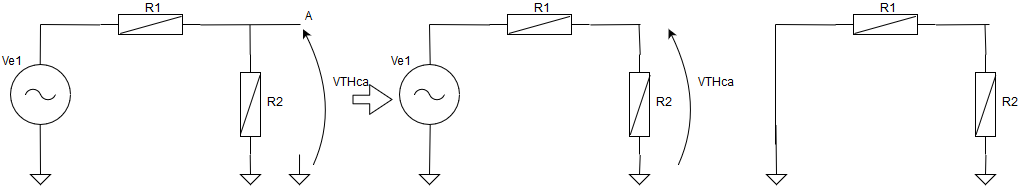
\includegraphics[scale=0.45]{Imagenes/6DisenoSistema/VTHcaMOD1.png}
    \caption{Voltaje Thevenin Alterno MOD 1}
	\label{fig:figure6}
\end{figure}
Para calcular el Voltaje de Thevenin, es necesario hacer un divisor de tensión en R2:\par 
\begin{center}
$\frac{Ve1 * R2}{R2 + R1} = VTHca$ \hspace{0.5cm} $\Rightarrow$\hspace{0.5cm} $\frac{0.1 * R2}{R2 + R1} = 0.05$ \hspace{0.5cm}$\Rightarrow$ \hspace{0.5cm}$0.05(R2 - R1) = 0$\\[0.5cm]
$\therefore R1  = R2$
\end{center}
Aquí se obtiene desde la información de RP3 que para que se cumpla lo solicitado las resistencias R1 y R2 deben ser iguales.\par

Para calcular la Red relajada de Thevenin apagamos la fuente de voltaje alterno:\par 
\begin{center}
 $\frac{R1 * R2}{R2 + R1} = ZTH_{ca}$\hspace{0.5cm} $\Rightarrow$\hspace{0.5cm} $\frac{R * R}{R + R}\geq 85 [\Omega]$\hspace{0.5cm} $\Rightarrow$ \hspace{0.5cm}$\frac{R}{2} \geq 85[\Omega]$\\[0.5cm]
$\therefore R\geq 170[\Omega]$   
\end{center}
Con los datos de RP3, buscamos el cumplimiento de los requisitos, obteniendo como resultado que tanto R1 como R2 deben ser mayores a 170 $[\Omega]$.\\[0.2cm] 

Por otro lado según RP3 cuando conectamos los módulos uno y dos debemos lograr que el punto de operación de nuestro diodo(1n4148) sea (0.72 [v],0.018 [A]), para ello analizamos el siguiente esquema:\par 
\begin{figure}[h!]
    \Centering
    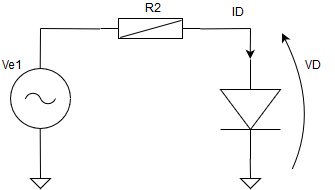
\includegraphics[scale=0.45]{Imagenes/6DisenoSistema/DISENORP2.png}
    \caption{Circuito diodo 1N4148}
	\label{fig:figure6}
\end{figure}

\newpage

Por LVK y tercer postulado podemos determinar el valor de R2:\par 
\[Ve2 = VR2 + VD \Rightarrow Ve2 = R2*IR2 + VD\Rightarrow R2 = \frac{Ve2 - VD}{IR2}\Rightarrow R2 = \frac{6.7[V]-0.72[V]}{0.018[A]}\]
\[\therefore R2 = 332.2[\Omega]\]

Por comodidad a la hora de formar el circuito definiremos tanto R2 como R1 con el valor de 330$[\Omega]$.\par 

La gráfica del diodo ID = f(VD) se obtendrá en el laboratorio, lo cual será especificado en la sección de estrategias de pruebas.\\[0.5cm]



\textbf{* Diseño de C1:}\\[0.1cm]
Según lo solicitado en RP2, la impedancia de C1 debe ser despreciable respecto a la resistencia vista por los terminales de salida, o bien, su resistencia equivalente Thévenin. Podemos notar que la impedancia más baja Thévenin que podemos obtener está dada por el mínimo de $ZTH_{ca}$; 170 $[\Omega]$ en este caso.
Por ende la impedancia del condensador (Zc1) dada por $\frac{1}{C}$ , debe cumplir :
Zc1 $<<$ 170 $[\Omega]$, tomamos el criterio de que 10 veces menor (mínimo) será un valor despreciable. Por esto, teniendo en cuenta que estamos trabajando con una frecuencia 3[KHz], el condensador fácilmente funcionará de la manera que necesitamos. Luego de dicho análisis definiremos $C1 = 10[\mu F]$.\par 


\subsubsection{Estrategias de Prueba MOD 1}
En el laboratorio, se comenzará montando el Módulo 1, según los valores de los componentes obtenidos en la subsección anterior. Además, se utilizará el generador de señales para obtener el voltaje Ve1, programado a 3[Khz] de frecuencia y 0.1 [V] de amplitud, centrada en 0, por otro lado, usaremos la fuente de voltaje continua para recrear la fuente Ve2, configurada a 6,7 [V]
En laboratorio, para ratificar que el sistema es lineal, lo cual podemos esperar, ya que utilizamos componentes lineales (pasado su transciente) y la suma de las fuentes se mantiene para diferentes valores de entrada se realizará una tabla donde se analizarán los valores de entrada y salida, realizando 4 incrementos discretos para la amplitud de cada fuente, y anotando los respectivos valores de las señales de entrada y salida.
 Comprobaremos además que los valores del condensador son despreciables analizando la existencia de desfase entre la entrada y salida por medio del osciloscopio.


\subsection{MOD 2}
\label{sec5.2.}
\subsubsection{Diseño Detallado del MOD 2}
\textbf{* Diseño de R4:}\\[0.2cm]
Dado RP5 y sabiendo que la resistencia dinámica del diodo en el punto indicado en RP4 es $RD = \frac{0.72[V]}{0.018[A]}$ podemos determinar que:\\[-0.2cm]

\begin{center}
$R4 \geq 10* RD$ \hspace{0.5cm} $\Rightarrow$ \hspace{0.5cm}$R4 \geq 10*40[\Omega]$\hspace{0.5cm}$\Rightarrow$\hspace{0.5cm}$\therefore R4 \geq 400[\Omega]$
\end{center}

\textbf{* Diseño de C2:}\\[0.2cm]
Según lo solicitado en RP2, la impedancia de C2 debe ser despreciable respecto a la resistencia vista por los terminales de salida, o bien, su resistencia equivalente Thévenin. Podemos notar que la impedancia más baja Thévenin que podemos obtener está dada por el mínimo de $ZT_{ca} << 170 $ $[\Omega]$ en este caso.
Por ende la impedancia del condensador (Zc1) dada por $\frac{1}{C}$ , debe cumplir :
$Zc1 << 170$ $[\Omega]$  , tomamos el criterio de que 10 veces menor (mínimo) será un valor despreciable. Por esto, teniendo en cuenta que estamos trabajando con una frecuencia 3[KHz], el condensador fácilmente funcionará de la manera que necesitamos. Luego de dicho análisis definiremos $C2 = 10[\mu F]$.\\[0.2cm]

\textbf{* Determinar factor k:}\\[0.2cm]
Para determinar K solo hace falta sacar el equivalente thevenin continuo, para luego compararlo con su expresión matemática relacionada.\par

\begin{figure}[h!]
    \Centering
    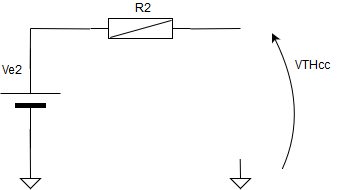
\includegraphics[scale=0.45]{Imagenes/6DisenoSistema/TheveninContinuo.png}
    \caption{Thevenin Voltaje Continuo MOD 1}
	\label{fig:figure6}
\end{figure}





Podemos decir que $VTH_{cc} = Ve2$ , por lo que según la ecuación de RF1:\par 
\begin{center}
    $Va = Ve2 + kVe1 \Rightarrow 6.75 [V] = 6.7 [V] + k +(0.1[V]) \Rightarrow \therefore k = 0.5$\par
    $Va = Ve2 + kVe1 \Rightarrow 6.65 [V] = 6.7 [V] + k +(-0.1[V]) \Rightarrow \therefore k = 0.5$\par
\end{center}
Se concluye que k como coeficiente tiene un valor fijo de 0.5.\\[0.2cm] 

\textbf{* Determinar factor n:}\\[0.1cm]

Para determinar n necesitamos una expresión que relación Ve1 con Vs1, en donde influya Ve2. Por lo visto anteriormente Ve2 esta directamente relacionado con la resistencia dinámica del diodo, como resultado si obtenemos un thevenin alterno para Vs1 nos queda la siguiente expresión:\par 
\begin{center}
    $n = \frac{Vs1}{Ve1}$ $\Rightarrow $ $n = \frac{Vs1 *\frac{330 // RD // 1K}{330 + 330// RD // 1K}}{Vs1}$ $\Rightarrow$ $n = \frac{253.8*RD}{330 + 253.8RD}$
\end{center}

Por otro lado tenemos la relación de Ve2 con VD:\Rpar 
\begin{center}
    $Ve2 = ID*R2 + VD$
\end{center}
Donde a su vez, si vemos la gráfica de ID =f(VD) podemos calcular RD implícitamente. Calculando RD podemos determinar un valor para n.\par







\subsubsection{Estrategias de Prueba MOD 2}
Primeramente comenzaremos analizando experimentalmente la curva característica de nuestro diodo, por medio de una tabla de valores. Realizaremos incrementos discretos de corriente mediante la variación de una resistencia (probablemente con ayuda de un potenciómetro), con una fuente fija. Con esto podremos predecir de manera más exacta los resultados ya que obtendremos su característica real.
Luego para probar el funcionamiento y la validez de los valores de componentes obtenidos a través del análisis matemático, según la sección de requisitos de prueba, realizaremos la construcción de circuito en el laboratorio, prestando principal atención en que los valores de salida del módulo 2 correspondan según lo especificado por la sección 4.2, principalmente comprobando el valor del punto de operación del diodo por otro lado verificar que la señal alterna de salida sea atenuada, al variar el valor de la fuente continua como se podría esperar.
Lo anterior será medido con ayuda de los Osciloscopios y Multímetros ocupados en el laboratorio.

\newpage

\section{Resultados del Laboratorio}

El trabajo experimental realizado en el laboratorio consiste en comprobar cada uno de los requisitos de prueba propuestos en el preinforme, los cuales suelen ser actualizados durante el desarrollo de la experiencia. Por lo anterior, en este informe se han actualizado los valores de ciertos componentes, basados en el correcto funcionamiento de los requisitos de prueba.

\vspace{0.4cm}

\begin{figure}[h]
    \Centering
    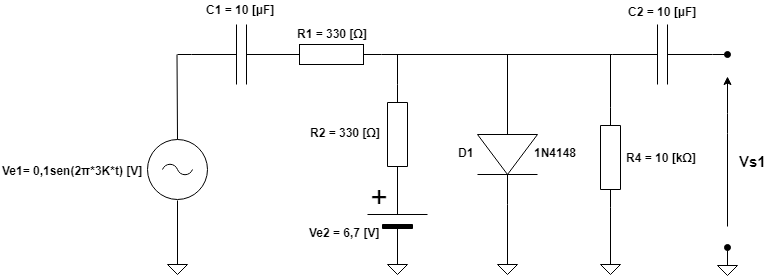
\includegraphics[scale=0.57]{Imagenes/7Resultados/circuites-inf3.png}
    \caption{Circuito implementado para análisis}
	\label{fig:figure9}
\end{figure}

\vspace{.4 cm}
En la Figura \ref{fig:figure9} podemos ver el circuito implementado para el desarrollo de esta experiencia, incluyendo los valores de cada componente.\\
Entendiendo que el circuito presentado corresponde a la unión del Módulo 1 (Figura \ref{fig:figure3}) y Módulo 2 (Figura \ref{fig:figure4}), se describirán las estrategias de resolución de los Requisitos de Prueba según el módulo que sea requerido.
\vspace{.2 cm}

\centering
\extrarowheight = -0.5ex
\renewcommand{\arraystretch}{2.25}
\begin{tabular}{p{0.1\textwidth} p{0.9\textwidth}}

\textbf{RP1} & Para este requisito se ha trabajado con dos diodos, 1n4148 y 1n4070, los cuales se examinaron por separado con la ayuda de una resistencia variable. Con el tester digital se midió el voltaje (V$_{D1}$) y la corriente (I$_{D1}$) que pasan por el diodo D1 mientras se variaba el voltaje continuo. En función de hacer una curva más detallada, en la cual sea evidente el comportamiento característico de los diodos, se realizó una gran cantidad de mediciones continuas de V$_{D1}$ e I$_{D1}$.  %(INSERTAR GRÁFICO Y TABLA DE MEDICIONES DE NICO)
\\ 

\end{tabular}


\begin{table}[h]
\resizebox{\textwidth}{!}{%
\begin{tabular}{|c|c|c|c|c|c|c|c|c|c|c|c|c|c|c|c|c|c|c|}
\hline
\textbf{VD {[}mV{]}} & 555 & 589 & 623 & 654 & 668 & 695 & 715 & 731 & 759 & 773 & 791 & 815 & 832 & 842 & 848 & 854 & 857 & 857 \\ \hline
\textbf{ID {[}mA{]}} & 0.5 & 1   & 2   & 3.8 & 5.1 & 9.1 & 14  & 20  & 40  & 56  & 99  & 175 & 260 & 378 & 500 & 769 & 840 & 895 \\ \hline
\end{tabular}%
}
\caption{Datos de Corriente y Voltaje por diodo 1N4007}
\label{my-label}
\end{table}

\newpage
\begin{figure}[h]
    \Centering
    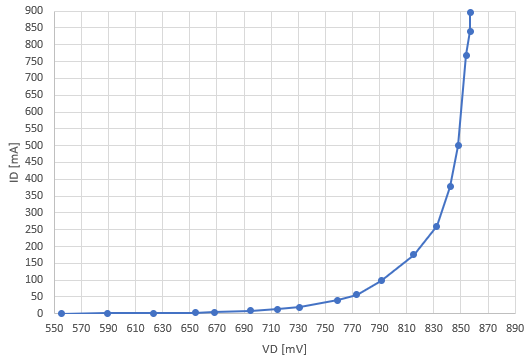
\includegraphics[scale=0.55]{Imagenes/7Resultados/diodo1n4007.png}
    \caption{Gráfico ID v/s VD Diodo 1N4007}
	\label{fig:figure10}
\end{figure}

\begin{table}[h]
\resizebox{\textwidth}{!}{%
\begin{tabular}{|c|c|c|c|c|c|c|c|c|c|c|c|c|c|c|c|c|c|}
\hline
\textbf{VD {[}mV{]}} & 585 & 618 & 649 & 680 & 720 & 730 & 735 & 786 & 797 & 807 & 826 & 844 & 892 & 937 & 943 & 961 & 997 \\ \hline
\textbf{ID {[}mA{]}} & 0.5 & 1   & 2   & 3.8 & 6   & 7   & 8   & 21  & 24  & 28  & 36  & 47  & 78  & 117 & 126 & 150 & 176 \\ \hline
\end{tabular}%
}
\caption{Datos de Corriente y Voltaje por diodo 1N4148}
\label{my-label}
\end{table}

\begin{figure}[h]
    \Centering
    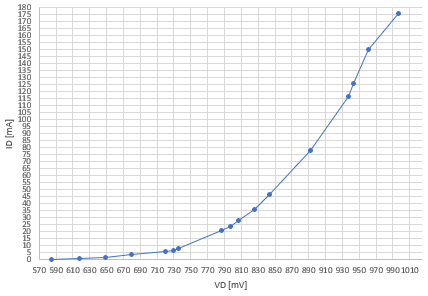
\includegraphics[scale=0.55]{Imagenes/7Resultados/diodo1n4148.png}
    \caption{Gráfico ID v/s VD Diodo 1N4148}
	\label{fig:figure10}
\end{figure}

\centering
\extrarowheight = -0.5ex
\renewcommand{\arraystretch}{2.25}
\begin{tabular}{p{0.1\textwidth} p{0.9\textwidth}}
\textbf{RP2} & Considerando el circuito completo, para poder demostrar que los valores de las capacitancias escogidas tienen carácter despreciable en el análisis de nuestra experiencia, debemos ver el desfase que pueden provocar los condensadores entre la señal alterna de entrada y la de salida. Por ello, se han medido las señales mencionadas, y podemos ver en la Figura \ref{fig:figure11} que no hay desfase entre ellas, por lo que el requisito queda demostrado. \\ 

\end{tabular}

\begin{figure}[h]
    \Centering
    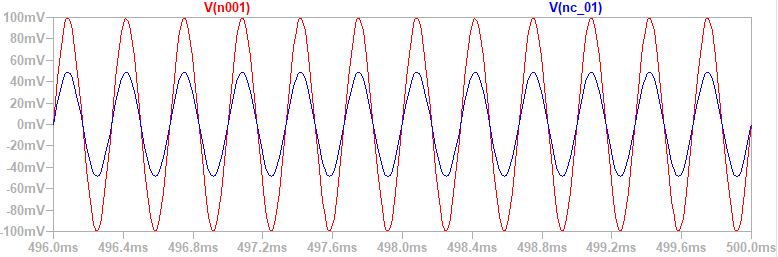
\includegraphics[scale=0.6]{Imagenes/7Resultados/ve1vs1.PNG}
    \caption{Señal alterna Ve1 y Ve2}
	\label{fig:figure11}
\end{figure}

\centering
\extrarowheight = -0.5ex
\renewcommand{\arraystretch}{2.25}
\begin{tabular}{p{0.1\textwidth} p{0.9\textwidth}}

\textbf{RP3} & Para este requisito se trabaja únicamente con el MOD 1, estableciendo un Voltaje Va, que se encuentra paralelo a la resistencia R2 y la fuente continua Ve2.\\
& Con la configuración propuesta en la descripción del requisito, medimos el voltaje alterno de salida en circuito abierto (Voltaje Thévenin VTca), como muestra la Figura \ref{fig:figure13}. El valor obtenido fue de \textbf{VTca = 46 [mV].} \\ 
\end{tabular}

\begin{figure}[h]
    \Centering
    \includegraphics[scale = 0.35]{Imagenes/7Resultados/vtca.png}
    \caption{Voltaje Thévenin alterno entre terminal a y tierra}
	\label{fig:figure13}
\end{figure}

\centering
\extrarowheight = -0.5ex
\renewcommand{\arraystretch}{2.25}
\begin{tabular}{p{0.1\textwidth} p{0.9\textwidth}}

& Para obtener la impedancia del equivalente Thévenin del MOD 1 sin apagar la fuente, utilizamos el modelo planteando en la Figura \ref{fig:figure14}.\\
\end{tabular}

\begin{figure}[h!]
    \Centering
    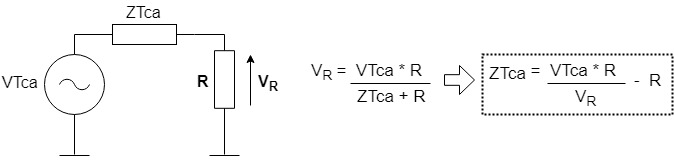
\includegraphics[scale=0.6]{Imagenes/6Analisis/divT.jpg}
    \caption{Divisor de Tensiones para $ZTH_{ca}$}
	\label{fig:figure14}
\end{figure}
\newpage
\centering
\extrarowheight = -0.5ex
\renewcommand{\arraystretch}{2.25}
\begin{tabular}{p{0.1\textwidth} p{0.9\textwidth}}

& Entonces, configurando el circuito con el modelo planteado, conectamos una resistencia R = 330 [$\Omega$], con voltaje V$_{R}$ = 30,4 [mV]. Por lo anterior, el resultado de ZTca para esta experiencia es: 
\[ ZTca = \frac{0,46 * 330}{0,304} - 330 = \mathbf{169,34 [\Omega]} \hspace{0.2cm} (\geq 85[\Omega] )
\]
\\ 

\textbf{RP4} & Para este requisitos hemos de trabajar con el circuito completo, es decir, ambos módulos conectados. \\
& Una vez configurado el circuito según la descripción de RP3, y obtenida la curva característica en la Figura \ref{fig:figure10}, con la fuente de poder variamos la corriente de entrada del tal forma que a través del diodo atraviesen los siguientes valores: \\
\end{tabular}

\begin{figure}[H]
\centering
\begin{minipage}[c]{0.4\linewidth}
\centering
    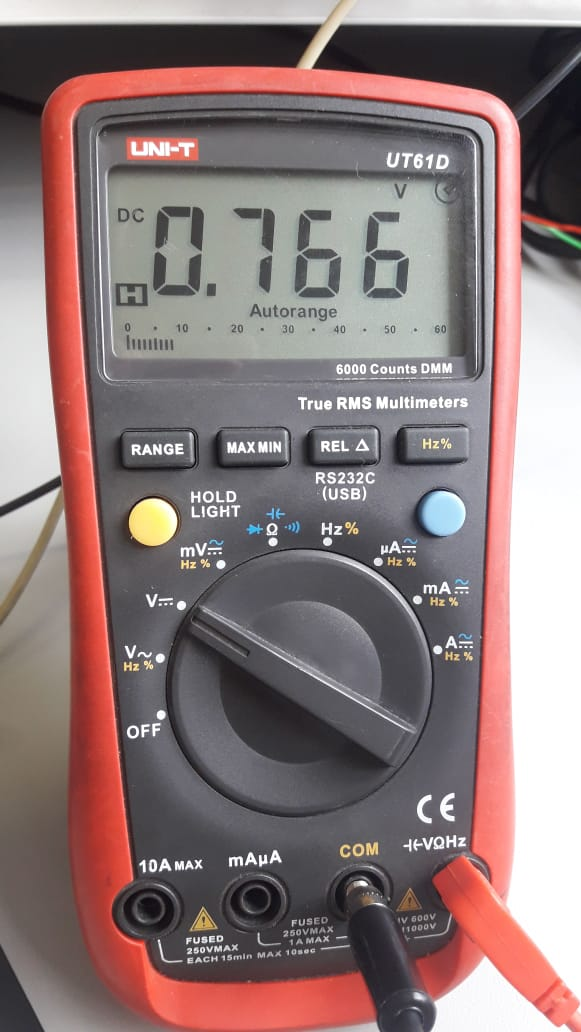
\includegraphics[scale=0.22]{Imagenes/7Resultados/Vdiodo.jpeg}
    \caption{Voltaje a través del diodo}
    \label{fig:figura1}
\end{minipage}
\hspace{0.25cm}
\begin{minipage}[c]{0.4\linewidth}
\centering
    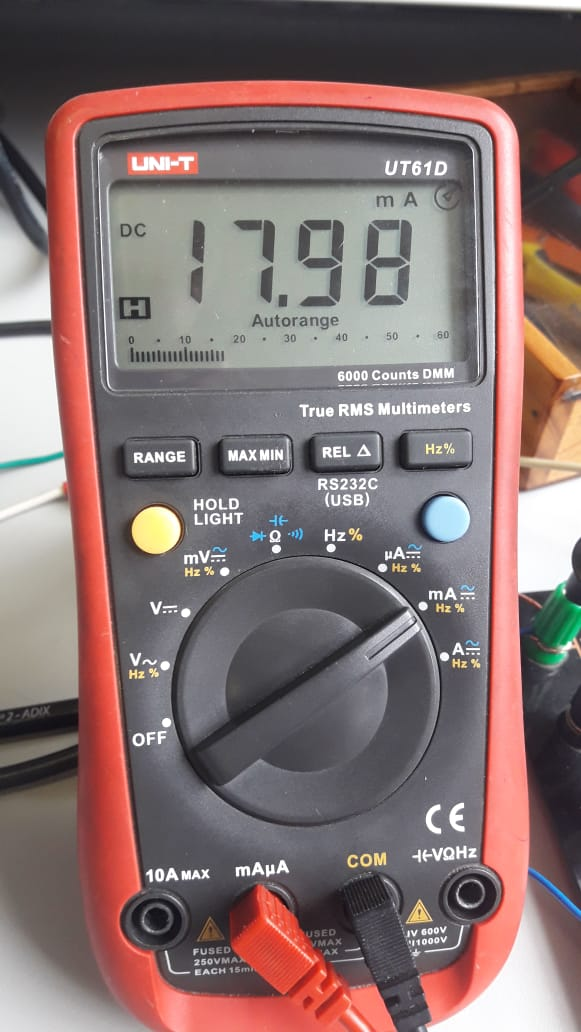
\includegraphics[scale=0.22]{Imagenes/7Resultados/Idiodo.jpeg}
    \caption{Corriente a través del diodo}
    \label{fig:figura2}
\end{minipage}
\end{figure}

\centering
\extrarowheight = -0.5ex
\renewcommand{\arraystretch}{2.25}
\begin{tabular}{p{0.1\textwidth} p{0.9\textwidth}}
& De esta forma queda definido el punto de operación Q con los valores presentados en las Figuras 11 y 12. 
\\ 

\textbf{RP5} & La resistencia dinámica del diodo en el punto Q se define de la siguiente manera:
\[ R_{D} = \frac{V_{DQ}}{I_{DQ}} = \frac{0.766}{0.01798} \approx 42,6 [\Omega]
\]
EL valor de R4 escogido es de 10[k$\Omega$], que cumple con $R4 >> 10 * R_{D}$.
\\

\textbf{RP6} & Para este requisito, se debe trabajar directamente con los requisitos funcionales, por lo tanto, para encontrar las constantes k y n nos dedicaremos a comprobar RF1 y RF2.
\end{tabular}

\newpage
\RaggedRight
\textbf{Prueba de Requisitos Funcionales} 
\\
\vspace{0.7cm}

\centering
\extrarowheight = -0.5ex
\renewcommand{\arraystretch}{2.25}
\begin{tabular}{p{0.1\textwidth} p{0.9\textwidth}}

\textbf{RF1} & En este requisito se trabaja sólo con el MOD1. Para observar la comparación de ambas señales, se realizó la simulación por LTSpice del MOD1, y de él se midió la señal entre los terminales de salida (ante la ausencia de dicha imagen, que se realizó en el laboratorio), del cual se obtuvo la señal que observamos en la Figura 15. Dicha señal corresponde al voltaje alterno de la señal Va, y esta oscila entre 125 [mV] y 223[mV]. 
\\
\end{tabular}

\begin{figure}[H]
\centering
\begin{minipage}[c]{0.4\linewidth}
\centering
    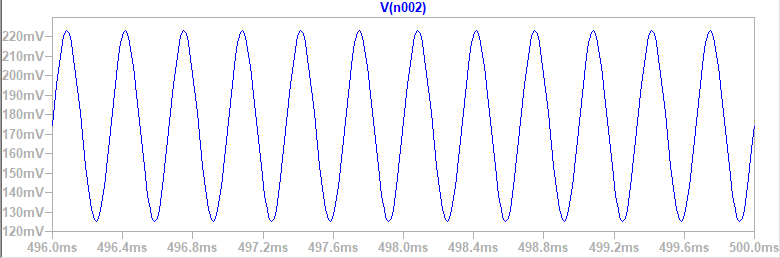
\includegraphics[scale=0.25]{Imagenes/7Resultados/Va.PNG}
    \caption{Señal de salida alterna de Va, MOD1}
    \label{fig:figura14}
\end{minipage}
\hspace{1.7cm}
\begin{minipage}[c]{0.4\linewidth}
\centering
    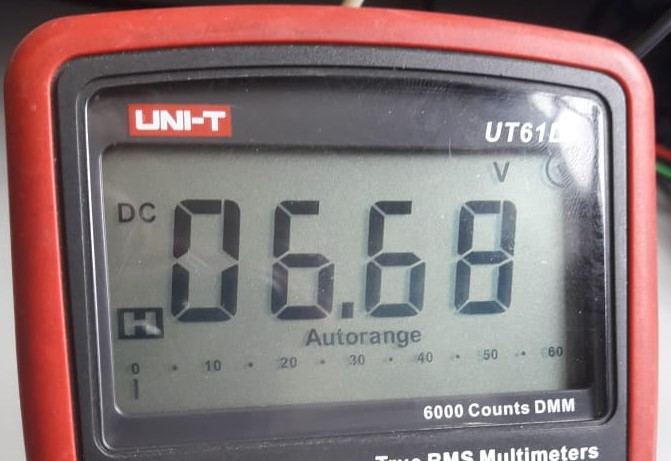
\includegraphics[scale=0.15]{Imagenes/7Resultados/Vcc.jpeg}
    \caption{Señal de salida continua de Va, MOD1}
    \label{fig:figura15}
\end{minipage}
\end{figure}

\centering
\extrarowheight = -0.5ex
\renewcommand{\arraystretch}{2.25}
\begin{tabular}{p{0.1\textwidth} p{0.9\textwidth}}
& La Figura 16 muestra el voltaje continuo medido con el tester digital para este módulo. \\
& De lo anterior, se concluye que $Va = 6,68 + 0,174sen(wt)[V]$, y podemos observar que el voltaje alterno de salida difiere en pequeñas magnitudes al voltaje alterno de entrada, por lo tanto, tomando en cuenta el detalle de los datos, el valor obtenido de la constante \textbf{k = 1,74}. 
\\
\end{tabular}
\vspace{0.6cm}

\centering
\extrarowheight = -0.5ex
\renewcommand{\arraystretch}{2.25}
\begin{tabular}{p{0.1\textwidth} p{0.9\textwidth}}
\textbf{RF2} & Este requisito define Vs1 = n*Ve1, para todo el circuito. Este requisito nos plantea un n variable, que dependerá de los valores que vayamos ingresando a la fuente continua Ve2.\\

& En la tabla \ref{Table2} se adjunta la "Tabla de Valores", obtenida luego de realizar varias mediciones al circuito, de la cual obtenemos distintos valores para n según vamos variando Ve2.
\end{tabular}

\begin{table}[h]
\centering
\caption{Tabla de Valores para n}
\label{Table2}
\begin{tabular}{@{}|c|c|c|c|c|@{}}
\toprule
Ve2 {[}V{]} & Idq {[}mA{]} & Vdq {[}V{]} & Vs1 pp {[}mV{]} & n \\ \midrule
6 & 0,756 & 5,34 & 2 & 0,01 \\
5 & 0,744 & 4,3 & 2,5 & 0,0125 \\
4 & 0,729 & 3,3 & 3 & 0,015 \\
3 & 0,710 & 2,36 & 4 & 0,02 \\
2 & 0,684 & 1,4 & 6 & 0,03 \\
1 & 0,624 & 0,499 & 16 & 0,08 \\
0,5 & 0,538 & 0,089 & 52 & 0,26 \\ \midrule
\textbf{0,18} & 0,157 & 0,021 & 97,8 & \textbf{0,489} \\ \bottomrule
\end{tabular}
\end{table}
\\ 

\centering
\extrarowheight = -0.5ex
\renewcommand{\arraystretch}{2.25}
\begin{tabular}{p{0.1\textwidth} p{0.9\textwidth}}
& De la tabla, destacamos el último valor de Ve2, que corresponde al ajuste del circuito que nos pide RP6, de modo que \textbf{ n = 0,489 $\approx$ 0,5}. Y con esta última prueba, quedan todos los Requisitos planteados durante el desarrollo de la experiencia y el informe verificados. \\
\end{tabular}
\\
\\
\\
\newpage

 
\newpage

\section{Conclusiones}
\RaggedRight

Para esta versión final del informe logramos arreglar todos los fallos cometidos en la primera fase en relación al desarrollo preinforme, principalmente generados al error de mezclar los Thévenin de alterna con los de continua,que esto desencadenó los cálculos erróneos para las resistencias además, nos percatamos luego que no habíamos comprobado después de realizar los cálculos en papel si esto cumplía con el RP3. De esta forma acumulamos varios problemas que no nos permitieron un buen desempeño durante la primera sesión del laboratorio.\\[0.3cm] \par
Luego de una completa reformulación de las ecuaciones, y cálculos de componentes , trabajando con inecuaciones y sin asignar valores hasta que no tuviéramos un sistema completo interceptado con el resto de los sistemas generados por cada requisito de prueba, haciendo este proceso en forma colectiva y también individual por cada miembro del grupo para ver si nos percatamos de nuevos errores en el proceso, logramos llegar a un correcto consenso y resultados correctos. 
Finalmente logramos solucionar todos los errores y llegar a una correcta realización de la experiencia.

\newpage
%%%%%%%%%%%%%%%%%%%%%%%%%%%%%%%%%%%%%%%%%%%%%%%%%%%%%%%%%%%%%%%

\end{document}
